\chapter{基本原理}
\newpage
\section{概要}
本章では, 本研究で具体的な焦点となる超音波の性質, エラストグラフィーの原理, 画像再構成手法, 低周波と生体組織の関係についての基礎的な原理について示す.

\section{超音波とは}
超音波は, 人の可聴域を超える20kHz以上の高周波の音波である. 超音波は運輸, 製造業, 建築, 水道, 農林水産, 食品そして医療に至るまで様々な分野で利用されている. 医療分野では診断装置, センサ, 通信機器, 補助具, 溶着などで多用されている. 

\section{超音波の性質}
医療機器では1\verb|〜|20MHzの超音波を使用しており, 超音波が生体内を伝播することで伝播経路における音響特性が変化する. この音響特性の分布の変化を解析することで, 生体内の組織の状態を観測できる. 以下で, 超音波と生体組織をの関係を述べるにあたり, 必要となる超音波の基本的な性質について述べる[10].
\begin{itemize}
\item{\bf 反射と屈折}
\\\ \ 超音波は異なる屈折率をもつ2つの物質を通過する際に, その境界面で反射・屈折を起こす. \figref{hansha} に音速$c_0$, 密度$\rho_0$の媒質から, 音速$c_1$, 密度$\rho_1$の媒質に超音波が入射する様子を示す. $\theta_0$, $\theta_1$はそれぞれ入射角, 屈折角を表す, また, 音速の異なる媒質に入射する際, 超音波の一部は境界面で反射する. \figref{hansha}の$\theta_0^{\prime}$で表されているのが反射角である. 入射角と反射角は等しい. また, 入射波と透過波の間ではSnellの法則が成り立つ.
\begin{equation}
\\ \dfrac{\sin\theta_0}{c_0} = \dfrac{\sin\theta_1}{c_1}
\end{equation}
生体組織では, 様々な音響特性をもつ物質が存在するため, 超音波パルスを与えた際に観察される複雑な波形の乱れは, 生体組織の境界面や音響特性などをはじめとした生体組織を特徴付ける, 様々な情報を含んでいる. 
\begin{figure}[H]
  \begin{center}
    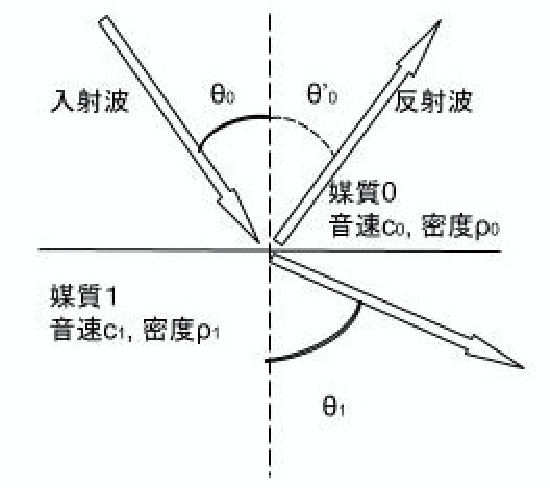
\includegraphics[width=75mm]{fig/hansha.pdf}
  \end{center}
  \caption{屈折率の異なる媒質間の境界面での超音波の挙動}
  \figlab{hansha}
\end{figure}
\item{\bf 音響インピーダンス}
\\\ \ 音響インピーダンスとは, 音波の伝播に際する通りにくさを表し, 電気工学でいう所の抵抗$R$であるというアナロジー的な説明が成されることが多い. 音響インピーダンスは物質ごとに固有な値であり, 振動数や振幅とは独立である. 音響インピーダンスは, 物質の密度,物質固有の音速cを用いて以下の式で表せる.
\begin{equation}
\label{eq.impeadance}
\\ $Z$ = \rho \times $c$
\end{equation}
音響インピーダンスの差異が超音波の反射や屈折のような現象を引き起こす. \figref{impeadance} に示すように, 境界面に対して超音波が直角に入射した際も, 音響インピーダンスの差異によって, 反射波, 透過波が生じる. \figref{impeadance} に音響インピーダンス$Z_0$, 密度$\rho_0$, 音速$c_0$から音響インピーダンス$Z_1$, 密度$\rho_1$, 音速$c_1$へ超音波が入射する様子を示す. 連続の式より, 反射率Rと透過率Tはそれぞれ(\ref{eq.R})式および(\ref{eq.T})式のように示せる.
\begin{equation}
\label{eq.R}
\\$R$= \dfrac{Z_2 - Z_1}{Z_2 + Z_1}
\end{equation}
\begin{equation}
\label{eq.T}
\\$T$= \dfrac{2Z_2}{Z_2 + Z_1}
\end{equation}
人体では, 骨などの音響インピーダンスの大きい部分では反射が生じるので, 超音波CTで得られる断層画像にも大きな影響を及ぼす. 
\begin{figure}[H]
  \begin{center}
    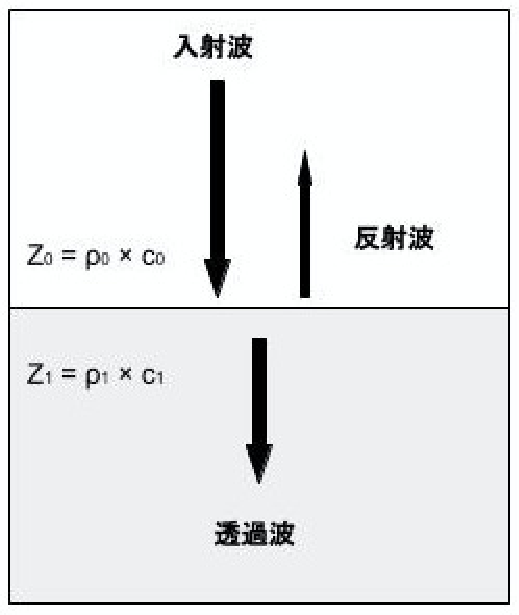
\includegraphics[width=75mm]{fig/impeadance.pdf}
  \end{center}
  \caption{音響インピーダンスの異なる媒質間の境界面での超音波の挙動}
  %[内閣府, 平成30年版高齢社会白書(全体版)]
  \figlab{impeadance}
\end{figure}
\item{\bf 音速と体積弾性率}
\\\ \ 音速は媒質を物理的に振動させることによって, 媒質の粗密が媒質中を伝播していく時の速度である. 生体内で伝搬する超音波は縦波で, その伝搬速度$c$は体積弾性率$K$および平均密度$\rho$を用いて, (\ref{eq.c})式のように表せる.
\begin{equation}
\label{eq.c}
\\$c$\ = \sqrt{\dfrac{K}{\rho}}
\end{equation}
\item{\bf 散乱}
\\\ \ 波長と同程度のサイズの媒質に入射すると回折が起こる. 生体内では, 反射, 屈折, 回折によって散乱が起こる. 波長に対して散乱体径が小さい場合は, 散乱強度は入射波の周波数の4乗に比例し, 光学におけるレイリー散乱のような振る舞いをする[11]. 波長と散乱体径が近い場合, ミー散乱に近い振る舞いをする. 
\item{\bf 減衰}
\\\ \ 減衰は, 散乱と吸収によって2点を結ぶ直線経路間のエネルギーの損失を表す. 生体組織は音速や密度が不均一に分布するため, 上述したように, 反射, 屈折, 回折などの現象が複雑に作用することで散乱場が生じる. 散乱は超音波のエネルギー損失を引き起こさない. 一方, 吸収は伝播中に超音波のエネルギーが熱に変換され, 音響エネルギーを失う.
\\\ \ 減衰率$\alpha$は, 初期音圧$p_0$, 伝播距離$x$, 減衰後の音圧$p$を用いて(\ref{eq.alpha})式のように表される.
\begin{equation}
\label{eq.alpha}
\\\alpha = \frac{20}{x}  \log{10} \frac{p_0}{p_1}
\end{equation}
生体内では, 減衰率$\alpha$は周波数$f$に依存し, 周波数$f$, 乗数$y$, 定数$\alpha_0$を用いて(\ref{eq.alpha_2})式のように表される.
\begin{equation}
\label{eq.alpha_2}
\\\alpha = \alpha_0f^y
\end{equation}
表\ref{table_soshiki}に, 人体の組織における減衰定数0と周波数fについてまとめる.

\begin{table}[htb]
\centering
\caption{人体の様々な組織における減衰率}
\label{table_soshiki}
\begin{tabular}{|c|c|c|}
\hline
組織 & 減衰率$\alpha_0$ & 計測周波数$f$[Hz]  \\ \hline
血液 & 0.2$\times$$10^{-7}$ &      1 \\ \hline
脳   & 1.05$\times$$10^{-7}$ &      3.4\\ \hline
肝臓  & 0.77$\times$$10^{-7}$ &     3 \\ \hline
脂肪 & 0.45$\times$$10^{-7}$ &     3.4 \\ \hline
頭蓋骨  & 24$\times$$10^{-7}$ &     1.8  \\ \hline
\end{tabular}
\end{table}

\end{itemize}
\section{エラストグラフィの原理}
医用画像の歴史は, ヴィルヘルム・コンラート・レントゲンの1895年のX線の発見にまで遡る. レントゲンは世界で初めてX線写真の撮影に成功したが,  生体にメスを入れることなく生体内部を可視化できることは, 非常に画期的なことであった. その後, 医用画像はディジタル計算機の登場により更に進化を遂げ, 今日ではX線画像だけでなく, 超音波画像, CT画像など医用画像の種類も多様化した. 超音波を用いた医用画像の取得は, 特にディジタル計算機の恩恵を受けた技術であり, 今後更なる発展が見込まれている. 以下では, エラストグラフィの原理について詳しく説明する. %[12].ここの引用はもう一度考えよう. 
\begin{itemize}
\item{\bf 生体組織の弾性と粘性}
\\生体組織はそれぞれの組織において様々な弾性と粘弾性を持っているため, 組織全体は不均一で複雑に入り組んだ構造となっている. そのため, 生体組織の力学的な挙動を記述する粘弾性モデルを仮定し, 弾性率を推定する.%https://www.jstage.jst.go.jp/article/mit/32/2/32_63/_pdf.
エラストグラフィでは, 組織を加圧あるいは加振することで粘性と弾性を評価し, 生体組織の硬さを計測する. 弾性を評価するにあたって, ヤング率は非常に重要なパラメータである. \figref{young}のように, 長軸方向に応力を加えた際に, フックの法則から(\ref{eq.young})式のように表せる. 
\begin{figure}[H]
  \begin{center}
    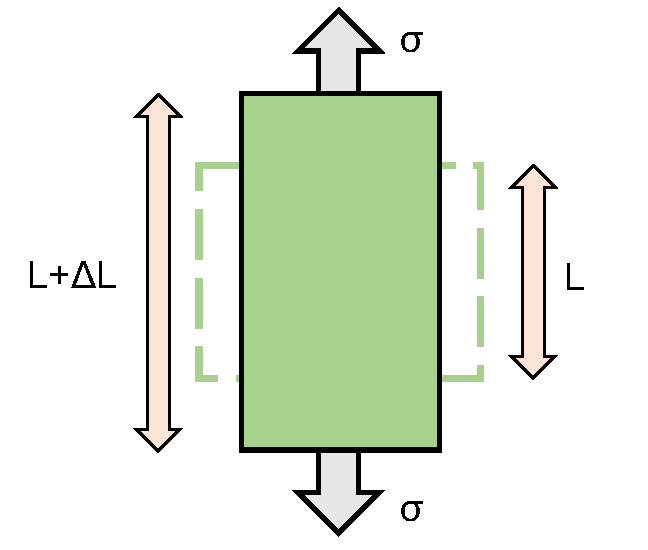
\includegraphics[width=60mm]{fig/ouryoku.pdf}
  \end{center}
  \caption{ヤング率と応力の関係}
  %[内閣府, 平成30年版高齢社会白書(全体版)]
  \figlab{young}
\end{figure}
\begin{equation}
\label{eq.young}
\\$E$ =  \dfrac{\sigma}{\epsilon}
\end{equation}
\end{itemize}



